\subsection{Подготовка данных}
\label{sec:experiment:data_preparation}



Как можно заметить, полученные данные являются как количественными, так и качественными. Количественные данные остаются
без изменений, для качественных(материал дома, качество ремонта) были введены числовые характеристики. 
Величина характеристики выставлялась в зависимотси от медианной стоимости всех объектов недвижимости с данной характеристикой.
Так, например, для материалов строительства были выставлены значения от 1 до 4 в следующем порядке: Панельный дом - 1,
монолитный - 2, каркасно-блочный - 3, кирпичный - 4.

Проведен анализ полученных данных. На рисунке~\ref{fig:experiment:hist_building_area} приведена гистограмма площадей
полученных объектов недвижимости, которая позволяет говорить что наиболее популярная недвижмиость имеет площадь от 40
до 60 квадратных метров.

\begin{figure}[!ht]
  \centering
  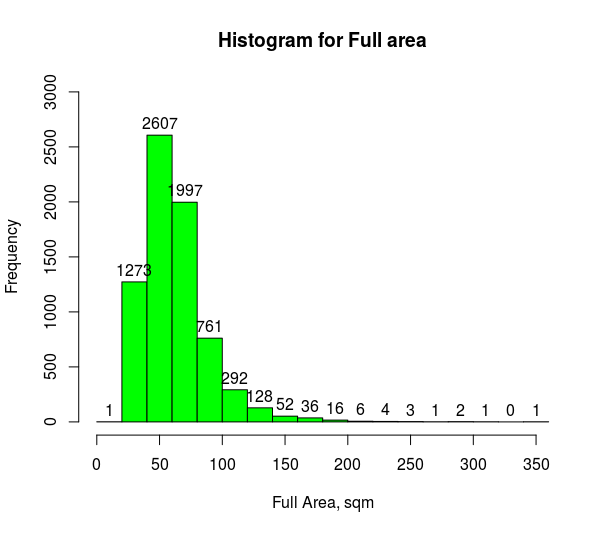
\includegraphics[scale=1]{hist_building_area.png} 
  \caption{Гистограмма площадей}
  \label{fig:experiment:hist_building_area}
\end{figure}

На рисунке~\ref{fig:experiment:barplot_bathrooms} приведена гистограмма санузлов
полученных объектов недвижимости, на которой видно что подавляющее большинство квартир имеют раздельный санузел.

\begin{figure}[!ht]
  \centering
  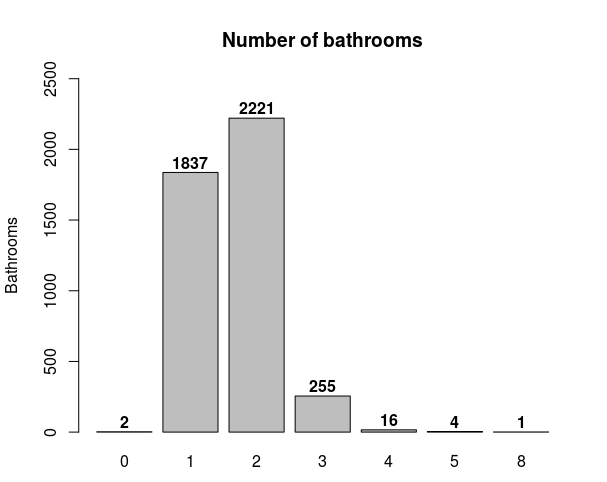
\includegraphics[scale=1]{barplot_bathrooms.png} 
  \caption{Гистограмма санузлов}
  \label{fig:experiment:barplot_bathrooms}
\end{figure}

На рисунке~\ref{fig:experiment:barplot_bedrooms} приведена гистограмма комнат
полученных объектов недвижимости, на которой видно что большинство квартир имеют 2 комнаты.

\begin{figure}[!ht]
  \centering
  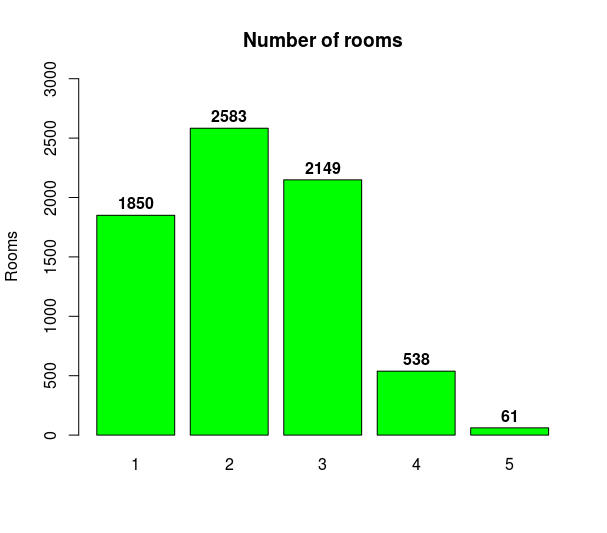
\includegraphics[scale=1]{barplot_bedrooms.png} 
  \caption{Гистограмма комнат}
  \label{fig:experiment:barplot_bedrooms}
\end{figure}

На рисунке~\ref{fig:experiment:hist_sold_price} можно увидеть, что большинство квартир продаются в диапазоне
цен от 40 до 100 тысяч долларов.

\begin{figure}[!ht]
  \centering
  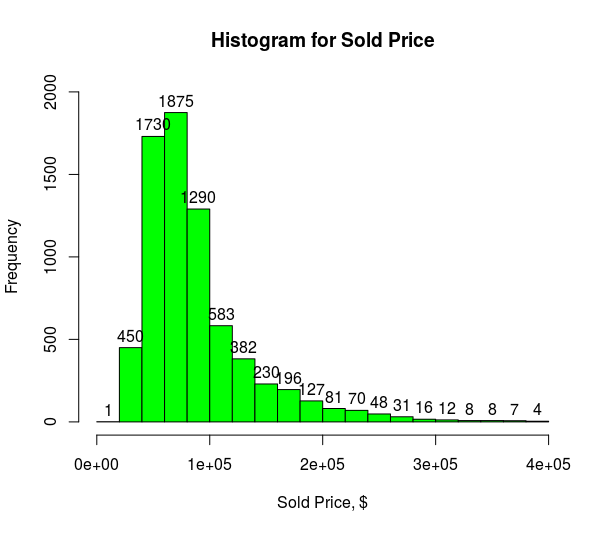
\includegraphics[scale=1]{hist_sold_price.png} 
  \caption{Гистограмма стоимости продажи}
  \label{fig:experiment:hist_sold_price}
\end{figure}
